%definira klasu dokumenta 
\documentclass[12pt]{report} 

%prostor izmedu naredbi \documentclass i \begin{document} se zove uvod. U njemu se nalaze naredbe koje se odnose na cijeli dokument

%osnovni LaTex ne može riješiti sve probleme, pa se koriste različiti paketi koji olakšavaju izradu željenog dokumenta
\usepackage[croatian]{babel} 
\usepackage{amssymb}
\usepackage{amsmath}
\usepackage{txfonts}
\usepackage{mathdots}
\usepackage{titlesec}
\usepackage{array}
\usepackage{lastpage}
\usepackage{etoolbox}
\usepackage{tabularray}
\usepackage{color, colortbl}
\usepackage{adjustbox}
\usepackage{geometry}
\usepackage[classicReIm]{kpfonts}
\usepackage{hyperref}
\usepackage{fancyhdr}

\usepackage{float}
\usepackage{setspace}
\restylefloat{table}


\patchcmd{\chapter}{\thispagestyle{plain}}{\thispagestyle{fancy}}{}{} %redefiniranje stila stranice u paketu fancyhdr

%oblik naslova poglavlja
\titleformat{\chapter}{\normalfont\huge\bfseries}{\thechapter.}{20pt}{\Huge}
\titlespacing{\chapter}{0pt}{0pt}{40pt}


\linespread{1.3} %razmak između redaka

\geometry{a4paper, left=1in, top=1in,}  %oblik stranice

\hypersetup{ colorlinks, citecolor=black, filecolor=black, linkcolor=black,	urlcolor=black }   %izgled poveznice


%prored smanjen između redaka u nabrajanjima i popisima
\newenvironment{packed_enum}{
	\begin{enumerate}
		\setlength{\itemsep}{0pt}
		\setlength{\parskip}{0pt}
		\setlength{\parsep}{0pt}
	}{\end{enumerate}}

\newenvironment{packed_item}{
	\begin{itemize}
		\setlength{\itemsep}{0pt}
		\setlength{\parskip}{0pt}
		\setlength{\parsep}{0pt}
	}{\end{itemize}}




%boja za privatni i udaljeni kljuc u tablicama
\definecolor{LightBlue}{rgb}{0.9,0.9,1}
\definecolor{LightGreen}{rgb}{0.9,1,0.9}

%Promjena teksta za dugačke tablice
\DefTblrTemplate{contfoot-text}{normal}{Nastavljeno na idućoj stranici}
\SetTblrTemplate{contfoot-text}{normal}
\DefTblrTemplate{conthead-text}{normal}{(Nastavljeno)}
\SetTblrTemplate{conthead-text}{normal}
\DefTblrTemplate{middlehead,lasthead}{normal}{Nastavljeno od prethodne stranice}
\SetTblrTemplate{middlehead,lasthead}{normal}

%podesavanje zaglavlja i podnožja

\pagestyle{fancy}
\lhead{Programsko inženjerstvo}
\rhead{Nestali ljubimci}
\lfoot{\textit{For All the Dogs}}
\cfoot{stranica \thepage/\pageref{LastPage}}
\rfoot{\today}
\renewcommand{\headrulewidth}{0.2pt}
\renewcommand{\footrulewidth}{0.2pt}


\begin{document} 
	
	
	
	\begin{titlepage}
		\begin{center}
			\vspace*{\stretch{1.0}} %u kombinaciji s ostalim \vspace naredbama definira razmak između redaka teksta
			\LARGE Programsko inženjerstvo\\
			\large Ak. god. 2023./2024.\\
			
			\vspace*{\stretch{3.0}}
			
			\huge \textit{Nestali ljubimci}\\
			\Large Dokumentacija, Rev. 1\\
			
			\vspace*{\stretch{12.0}}
			\normalsize
			Grupa: \textit{For All the Dogs}\\
			Voditelj: \textit{Andrija Merlin}\\
			
			
			\vspace*{\stretch{1.0}}
			Datum predaje: \textit{17. 11. 2023.}\\
	
			\vspace*{\stretch{4.0}}
			
			Nastavnik: \textit{Alan Jović}\\
		
		\end{center}

	
	\end{titlepage}

	
	\tableofcontents


	\chapter{Dnevnik promjena dokumentacije}
		
		\begin{longtblr}[
				label=none
			]{
				width = \textwidth, 
				colspec={|X[2]|X[13]|X[3]|X[3]|}, 
				rowhead = 1
			}
			\hline
			\textbf{Rev.}	& \textbf{Opis promjene/dodatka} & \textbf{Autori} & \textbf{Datum}\\[3pt] \hline
			0.1 & Napravljen predložak & Božo Đerek & 26.10.2023. 		\\[3pt] \hline 
			0.2	& Opis projektnog zadatka\newline Nefunkcionalni zahtjevi, dio funkcionalnih zahtjeva & Božo Đerek,\newline Lucija Lovrić & 27.10.2023. 	\\[3pt] \hline 
			0.5 & Dodan \textit{Use Case} dijagram i jedan sekvencijski dijagram, funkcionalni i nefunkcionalni zahtjevi i dodatak A & * & 25.08.2013. \\[3pt] \hline 
			0.6 & Arhitektura i dizajn sustava, algoritmi i strukture podataka & * & 26.08.2013. \\[3pt] \hline 
			0.8 & Povijest rada i trenutni status implementacije,\newline Zaključci i plan daljnjeg rada & * & 28.08.2013. \\[3pt] \hline 
			0.9 & Opisi obrazaca uporabe & * & 07.09.2013. \\[3pt] \hline 
			0.10 & Preveden uvod & * & 08.09.2013. \\[3pt] \hline 
			0.11 & Sekvencijski dijagrami & * & 09.09.2013. \\[3pt] \hline 
			0.12.1 & Započeo dijagrame razreda & * & 10.09.2013. \\[3pt] \hline 
			0.12.2 & Nastavak dijagrama razreda & * & 11.09.2013. \\[3pt] \hline 
			\textbf{1.0} & Verzija samo s bitnim dijelovima za 1. ciklus & * & 11.09.2013. \\[3pt] \hline 
			1.1 & Uređivanje teksta -- funkcionalni i nefunkcionalni zahtjevi & * \newline * & 14.09.2013. \\[3pt] \hline 
			1.2 & Manje izmjene:Timer - Brojilo vremena & * & 15.09.2013. \\[3pt] \hline 
			1.3 & Popravljeni dijagrami obrazaca uporabe & * & 15.09.2013. \\[3pt] \hline 
			1.5 & Generalna revizija strukture dokumenta & * & 19.09.2013. \\[3pt] \hline 
			1.5.1 & Manja revizija (dijagram razmještaja) & * & 20.09.2013. \\[3pt] \hline 
			\textbf{2.0} & Konačni tekst predloška dokumentacije  & * & 28.09.2013. \\[3pt] \hline 
			&  &  & \\[3pt] \hline	
		\end{longtblr}
	\chapter{Opis projektnog zadatka}

		Gubitak kućnog ljubimca može biti jedna od emocionalno najtežih stvari kroz koje vlasnik može proći. Ponekad se dogodi da ljubimac odluta od kuće zbog znatiželje, iznenadnog događaja koji je u njima probudio strah... U tom slučaju, vlasniku je prioritet brzo pronaći mezimca kako bi bio na sigurnom u svom domu.
		
		Naša aplikacija je namijenjena onima koji su izgubili kućnog ljubimca, onima koji žele pomoći drugima u pronalasku svojih krznenih prijatelja pa i skloništima koji pod svoje primaju odlutale prestrašene životinje. Svi zainteresirani za dobrobit ovih ljubimaca imaju direktan pristup svim informacijama o njima. Značaj aplikacije za zajednicu je da može doprinijeti smanjenju broja napuštenih ljubimaca i time olakšati rad skloništima za životinje te promovirati svijest o izgubljenim ljubimcima. \\
		
		Ova korisna i jednostavna responzivna aplikacija pomoći će u rješavanju ovog problema mnogim korisnicima aplikacije.\\
		
		Cilj ovog projekta je razviti programsku potporu za stvaranje web aplikacije „Nestali ljubimci“. U opseg projektnog zadatka ulazi izrada web platforme koja podržava registraciju korisnika/skloništa, postavljanje, pretragu i ažuriranje postojećih oglasa te ima pridruženu bazu podataka koja pohranjuje korisne informacije. Sustav treba podržavati rad više korisnika u stvarnom vremenu. Manipuliranje podacima obavlja se kroz sučelje baze podataka tako da nije potreban administrator.\\
		
		Web aplikacija je namijenjena za 3 vrste korisnika; neregistriranog korisnika, registriranog korisnika te skloništima za životinje (specijalni tip registriranog korisnika).
		
		\underline{Neregistrirani korisnik} ima mogućnost pregledavanja i pretraživanja nestalih kućnih ljubimaca. Klikom na sliku nestale životinje, znatiželjnom korisniku otvaraju se informacije o njoj: vrsta, ime, datum i sat nestanka, lokacija nestanka, boja, starost, tekstni opis. Uz to dostupne su do 3 slike te životinje kako bi ju tragač lakše pronašao, a ako bi došlo do novih informacija ili pronalaska ljubimca dostupni su i kontakt podaci vlasnika. Neregistrirani korisnik bi se trebao registrirati ako bi poželio sudjelovati u potrazi i ostvariti komunikaciju s dotičnim vlasnikom. Za registraciju su potrebni sljedeći podaci:
		
		\begin{packed_item}
			\item adresa e-pošte
			\item broj telefona
			\item korisničko ime
			\item lozinka
			\item ime i prezime/naziv skloništa
		\end{packed_item}
		
		\underline{Registrirani korisnik} ima širi spektar mogućnosti unutar aplikacije. On može, uz pregledavanje i pretraživanje, postaviti oglas o nestalom ljubimcu, izmijeniti i ukloniti ga pa i sudjelovati u komunikaciji s drugim registriranim korisnicima.\\
		
		Postoje 4 kategorije oglasa:
		
		\begin{packed_item}
			\item Za ljubimcem se traga (početna postavka oglasa)
			\item Ljubimac je sretno pronađen
			\item Ljubimac nije nađen, ali se za njim ne traga aktivno
			\item Ljubimac je pronađen pod nesretnim okolnostima
		\end{packed_item}
		
		\underline{Skloništa za životinje} su vrsta registriranih korisnika koji oglašavaju životinje koje su pronašli te se nalaze kod njih.
		
		\eject
		
		\section{Postojeća slična rješenja}
		
		Model našeg projekta moći će se koristiti na globalnoj razini zbog svoje jednostavnosti i prilagodljivosti lokaciji. Već postoji nekoliko web stranica s kojima dijelimo zajednički cilj poput \textit{PetFinder}, \textit{LostMyDoggie.com}, \textit{PawBoost} i \textit{Petco Love}.
		
		\begin{packed_item}		
		
			\item \textit{PetFinder} je naširoko poznata baza podataka za udomljavanje životinja, a imaju i odjeljak za tražene i pronađene kućne ljubimce.
		
			\item \textit{LostMyDoggie.com} je web stranica koja je napravljena specijalno kako bi pomogla vlasnicima pronaći svoje kućne ljubimce.
		
			\item \textit{PawBoost} je platforma koja omogućuje korisnicima da prijave nestanak ljubimca nakon čega stranica stvori oglas na Facebooku čime se širi vijest o nestanku ljubimca.
		
			\item \textit{Petco Love} je web stranica na kojoj se može prijaviti nestanak, ali i pronalazak kućnog ljubimca. Pri tome se šalju i slike ljubimca te se koristi \textit{facial recognition technology} za identificiranje ljubimaca.
		
		\end{packed_item}
		
		U našoj regiji se trenutno ipak nešto više komunicira preko raznih Facebook grupa, lokalnih skloništa za životinje, oglašavanja preko veterinara i lijepljenjem papira s oglasom po ulicama.\\
		
		%unos slike
		\begin{figure}[H]
			
\includegraphics[scale=0.5]{slike/pawBoost.PNG} 
			\centering
			\caption{oglas platforme PawBoost}
			\label{pawBoost}
		\end{figure}
		
		\begin{figure}[H]
			
\includegraphics[scale = 0.4]{slike/petcoLove.PNG} 
			\centering
			\caption{usluge koje nudi platforma PetcoLove}
			\label{petcoLove}
		\end{figure}
		
		\begin{figure}[H]
			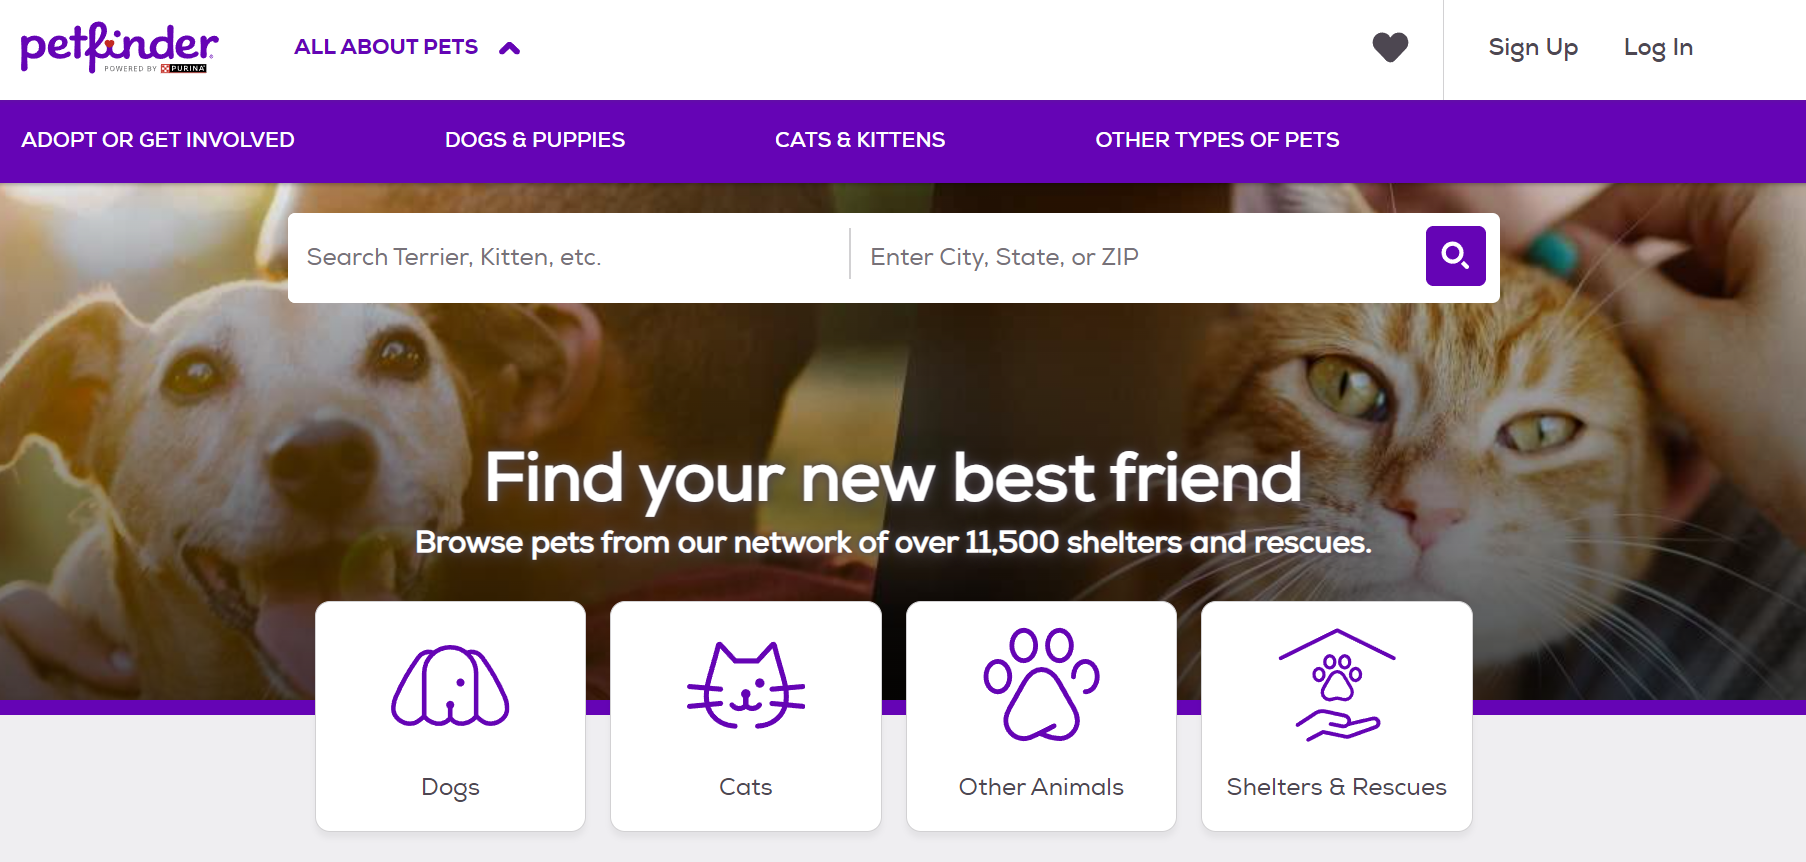
\includegraphics[scale = 0.5]{slike/petFinder.PNG} 
			\centering
			\caption{web stranica platforme PetFinder}
			\label{petcoLove}
		\end{figure}
		
		\pagebreak
		
		
		\section{Moguće prilagodbe i nadogradnje rješenja}
		
		\begin{packed_item}
		
			\item Lokaliziranjem aplikacije ona bi postala dostupna i korisnicima u zemljama s drugim jezicima, zakonima i običajima.
			
			\item Osnovni princip naše aplikacije se može primijeniti i na razne izgubljene predmete. Naša aplikacija je svojevrsni \textit{lost and found} (rekonstrukcija nestanka?) primijenjen na ljubimce.
			
			\item Nakon početne implementacije, neke od mogućih projektnih nadogradnji uključuju i \textit{real time chat} opciju. Korisnici bi mogli međusobno privatno komunicirati i dijeliti razne informacije o nestalim ljubimcima. Registrirani korisnik s informacijama koje mogu pomoći vlasniku izgubljenog ljubimca mogao bi privatno kontaktirati vlasnika koji je objavio oglas.
			
			\item Uvođenje naprednih algoritama za prepoznavanje životinja putem fotografija olakšalo bi i ubrzalo pronalazak.
			
			\item Povezivanje podataka aplikacije, skloništa i veterinarskih klinika dodatno bi poboljšalo potragu.
			
			\item Na web aplikaciji bi mogla postojati mogućnost donacije sredstava lokalnim skloništima za životinje.
			
		\end{packed_item}
		
		\eject
	\chapter{Specifikacija programske potpore}
		
	\section{Funkcionalni zahtjevi}
			
			\iffalse
			\textit{Navesti \textbf{dionike} koji imaju \textbf{interes u ovom sustavu} ili  \textbf{su nositelji odgovornosti}. To su prije svega korisnici, ali i administratori sustava, naručitelji, razvojni tim.}\\
				
			\textit{Navesti \textbf{aktore} koji izravno \textbf{koriste} ili \textbf{komuniciraju sa sustavom}. Oni mogu imati inicijatorsku ulogu, tj. započinju određene procese u sustavu ili samo sudioničku ulogu, tj. obavljaju određeni posao. Za svakog aktora navesti funkcionalne zahtjeve koji se na njega odnose.}\\
			\fi
			
			\noindent \textbf{Dionici:}
			
			\begin{packed_enum}
				
				\item Neregistrirani korisnik
				\item Registrirani korisnik			
				\item Sklonište za životinje
				\item Razvojni tim
				\item Naručitelji
				
			\end{packed_enum}
			
			\noindent \textbf{Aktori i njihovi funkcionalni zahtjevi:}
			
			
			\begin{packed_enum}
				\item  \underbar{Neregistrirani korisnik (inicijator) može:}
				
				\begin{packed_enum}
					
					\item pregledavati i pretraživati oglašene nestale kućne ljubimce i skloništa za životinje
					\item odabrati nekog od kućnih ljubimaca, čime se otvara mogućnost detaljnijeg pregleda informacija o njemu kao i pregled komunikacije oko potrage za ljubimcem
					\item registrirati se, stvoriti novi korisnički račun za koji su mu potrebni e-pošta, broj telefona, korisničko ime, lozinka te opcionalno (u slučaju registracije kao sklonište) naziv skloništa
					
				\end{packed_enum}
			
				\item  \underbar{Registrirani korisnik (inicijator) može:}
				
				\begin{packed_enum}
					
					\item sve što može neregistrirani korisnik
					\item prijaviti se u sustav
					\item postaviti, izmijeniti i ukloniti oglas o nestalom kućnom ljubimcu
					\item sudjelovati u komunikaciji oko potrage za ljubimcem
					\item pretraživati neaktivne oglase
					
				\end{packed_enum}
			
			\item  \underbar{Sklonište (inicijator) može:}
				
				\begin{packed_enum}
				
					\item sve što može registrirani korisnik
					\item oglašavati pronađene životinje koje se nalazi u prostoru skloništa pomoću kategorije oglasa "\textit{u skloništu}"
					
				\end{packed_enum}
			
			\item  \underbar{Baza podataka (sudionik):}
				
				\begin{packed_enum}
					
					\item pohranjuje sve podatke korisnika
					\item pohranjuje sve podatke vezane uz oglase
					
				\end{packed_enum}
			\end{packed_enum}
			
			\eject 
			
			
				
			\subsection{Obrasci uporabe}
				
				\subsubsection{Opis obrazaca uporabe}

					\noindent \underbar{\textbf{UC1 - Registracija}}
					\begin{packed_item}
	
						\item \textbf{Glavni sudionik:} Neregistrirani korisnik
						\item  \textbf{Cilj:} Stvoriti korisnički račun za pristup sustavu
						\item  \textbf{Sudionici:} Baza podataka
						\item  \textbf{Preduvjet:} -
						\item  \textbf{Opis osnovnog tijeka:}
						
						\item[] \begin{packed_enum}
	
							\item Korisnik odabire opciju za registraciju
							\item Korisnik unosi potrebne korisničke podatke
							\item Korisnik prima obavijest o uspješnoj registraciji
						\end{packed_enum}
						
						\item  \textbf{Opis mogućih odstupanja:}
						
						\item[] \begin{packed_item}
	
							\item[2.a] Odabir već zauzetog korisničkog imena i/ili e-maila, unos korisničkog podatka u nedozvoljenom formatu ili pružanje neispravnog e-maila
							\item[] \begin{packed_enum}
								
								\item Sustav obavještava korisnika o neuspjelom upisu i vraća ga na stranicu za registraciju
								\item Korisnik mijenja potrebne podatke te završava unos ili odustaje od registracije
								
							\end{packed_enum}
							
						\end{packed_item}
					\end{packed_item}
					
					\noindent \underbar{\textbf{UC2 - Prijava u sustav}}
					\begin{packed_item}
	
						\item \textbf{Glavni sudionik:} Neprijavljeni registrirani korisnik
						\item  \textbf{Cilj:} Dobiti pristup mogućnostima registriranih korisnika
						\item  \textbf{Sudionici:} Baza podataka
						\item  \textbf{Preduvjet:} Registracija
						\item  \textbf{Opis osnovnog tijeka:}
						
						\item[] \begin{packed_enum}
	
							\item Unos korisničkog imena i lozinke
							\item Provjera ispravnosti unesenih podataka
							\item Pristup korisničkim funkcijama
						\end{packed_enum}
						
						\item  \textbf{Opis mogućih odstupanja:}
						
						\item[] \begin{packed_item}
	
							\item[2.a] Neispravno korisničko ime/lozinka
							\item[] \begin{packed_enum}
								
								\item Sustav obavještava korisnika o neuspjeloj prijavi i vraća ga na stranicu za prijavu
								
							\end{packed_enum}
							
						\end{packed_item}
					\end{packed_item}
					
					\noindent \underbar{\textbf{UC3 - Pregled korisničkih podataka}}
					\begin{packed_item}
	
						\item \textbf{Glavni sudionik:} Registrirani korisnik/sklonište za životinje
						\item  \textbf{Cilj:} Pregledati korisničke podatke
						\item  \textbf{Sudionici:} Baza podataka
						\item  \textbf{Preduvjet:} Prijava u sustav
						\item  \textbf{Opis osnovnog tijeka:}
						
						\item[] \begin{packed_enum}
	
							\item Korisnik odabire opciju za pregled korisničkih podataka
							\item Aplikacija prikazuje podatke korisnika
						\end{packed_enum}
					\end{packed_item}
					
					\noindent \underbar{\textbf{UC4 - Promjena korisničkih podataka}}
					\begin{packed_item}
	
						\item \textbf{Glavni sudionik:} Registrirani korisnik/sklonište za životinje
						\item  \textbf{Cilj:} Promijeniti korisničke podatke
						\item  \textbf{Sudionici:} Baza podataka
						\item  \textbf{Preduvjet:} Prijava u sustav
						\item  \textbf{Opis osnovnog tijeka:}
						
						\item[] \begin{packed_enum}
	
							\item Korisnik pregledava korisničke podatke
							\item Korisnik odabire opciju za promjenu podataka
							\item Korisnik mijenja željene podatke i potvrđuje izmjenu
							\item Baza podataka se ažurira
						\end{packed_enum}
						
						\item \textbf{Opis mogućih odstupanja:} 
						
						
						\item[] \begin{packed_item}
	
							\item[3.a] Korisnik je promijenio svoje podatke, ali ih je zaboravio spremiti
							\item[] \begin{packed_enum}
								
								\item Sustav obavještava korisnika o neuspjeloj promjeni podataka
								\item Korisnik sprema izmijenjene podatke
								
								\end{packed_enum}
						\end{packed_item}
					\end{packed_item}
					
					\noindent \underbar{\textbf{UC5 - Brisanje korisničkog računa}}
					\begin{packed_item}
	
						\item \textbf{Glavni sudionik:} Registrirani korisnik/sklonište za životinje
						\item  \textbf{Cilj:} Obrisati korisnički račun
						\item  \textbf{Sudionici:} Baza podataka
						\item  \textbf{Preduvjet:} Prijava u sustav
						\item  \textbf{Opis osnovnog tijeka:}
						
						\item[] \begin{packed_enum}
	
							\item Korisnik pregledava korisničke podatke
							\item Korisnik odabire opciju za brisanje korisničkog računa
							\item Korisnik potvrđuje odabir
							\item Baza podataka se ažurira
						\end{packed_enum}
					\end{packed_item}
					
					\noindent \underbar{\textbf{UC6 - Pretraživanje i pregled oglasa o nestalim ljubimcima}}
					\begin{packed_item}
	
						\item \textbf{Glavni sudionik:} Korisnik
						\item  \textbf{Cilj:} Pregledati oglase nestalih ljubimaca
						\item  \textbf{Sudionici:} Baza podataka
						\item  \textbf{Preduvjet:} -
						\item  \textbf{Opis osnovnog tijeka:}
						
						\item[] \begin{packed_enum}
	
							\item Korisniku se prikazuju oglasi o nestalim ljubimcima
							\item Oglasi se mogu filtrirati po relevantnim podacima, s tim da su neaktivni oglasi vidljivi samo registriranim korisnicima
							\item Prikaz filtriranih oglasa
						\end{packed_enum}
						
						\item  \textbf{Opis mogućih odstupanja:}
						
						\item[] \begin{packed_item}
	
							\item[2.a] Ne postoji oglas koji odgovara postavljenom filtru
							\item[] \begin{packed_enum}
								
								\item Sustav korisniku prikazuje odgovarajuću poruku
								
							\end{packed_enum}
							
						\end{packed_item}
					\end{packed_item}
					
					\noindent \underbar{\textbf{UC7 - Postavljanje oglasa o nestalom ljubimcu}}
					\begin{packed_item}
	
						\item \textbf{Glavni sudionik:} Registrirani korisnik
						\item  \textbf{Cilj:} Postaviti oglas o nestalom ljubimcu
						\item  \textbf{Sudionici:} Baza podataka
						\item  \textbf{Preduvjet:} Prijava u sustav
						\item  \textbf{Opis osnovnog tijeka:}
						
						\item[] \begin{packed_enum}
	
							\item Korisnik odabire opciju postavljanja oglasa
							\item Korisnik dobiva mogućnost unošenja sljedećih kategorija podataka o ljubimcu:
								
								\item[] \begin {packed_enum}
									\item vrsta
									\item ime na koje se odaziva
									\item datum i sat nestanka
									\item lokacija nestanka
									\item boja
									\item starost
									\item tekstni opis
									\item do 3 slike
								\end{packed_enum}
							
							\item Ako je korisnik sklonište, postavlja kategoriju oglasa "\textit{u skloništu}"
							\item Korisnik odabire opciju za objavljivanje i njegov oglas postaje vidljiv drugima
						\end{packed_enum}
					\end{packed_item}
					
					\noindent \underbar{\textbf{UC8 - Izmjena oglasa o nestalom ljubimcu}}
					\begin{packed_item}
	
						\item \textbf{Glavni sudionik:} Registrirani korisnik
						\item  \textbf{Cilj:} Izmijeniti oglas o nestalom ljubimcu
						\item  \textbf{Sudionici:} Baza podataka
						\item  \textbf{Preduvjet:} Prijava u sustav
						\item  \textbf{Opis osnovnog tijeka:}
						
						\item[] \begin{packed_enum}
	
							\item Korisnik odabire opciju izmjene svog oglasa
							\item Korisnik mijenja željene podatke, dostupna mu je i promjena kategorije oglasa u neku od sljedećih:
								
								\item[] \begin{packed_enum}
									\item za ljubimcem se traga (\textit{pretpostavljeno})
									\item ljubimac je sretno pronađen
									\item ljubimac nije pronađen, ali se za njim više aktivno ne traga
									\item ljubimac je pronađen uz nesretne okolnosti
								\end{packed_enum}
							\item Korisnik potvrđuje izmjene
						\end{packed_enum}
					\end{packed_item}
					
					\noindent \underbar{\textbf{UC9 - Uklanjanje oglasa o nestalom ljubimcu}}
					\begin{packed_item}
	
						\item \textbf{Glavni sudionik:} Registrirani korisnik
						\item  \textbf{Cilj:} Ukloniti oglas o nestalom ljubimcu
						\item  \textbf{Sudionici:} Baza podataka
						\item  \textbf{Preduvjet:} Prijava u sustav
						\item  \textbf{Opis osnovnog tijeka:}
						
						\item[] \begin{packed_enum}
	
							\item Korisnik odabire opciju uklanjanja svog oglasa
							\item Uklonjeni oglas i sva pripadna komunikacija nestaje iz popisa vidljivih oglasa, ali se ne briše iz baze podataka
						\end{packed_enum}
					\end{packed_item}
					
					\noindent \underbar{\textbf{UC10 - Oglašavanje nestalih ljubimaca u skloništu}}
					\begin{packed_item}
	
						\item \textbf{Glavni sudionik:} Sklonište za životinje
						\item  \textbf{Cilj:} Postaviti oglas o nestalom ljubimcu u skloništu radi pronalaska vlasnika
						\item  \textbf{Sudionici:} Baza podataka
						\item  \textbf{Preduvjet:} Prijava u sustav
						\item  \textbf{Opis osnovnog tijeka:}
						
						\item[] \begin{packed_enum}
	
							\item Sklonište za životinje postavlja oglas kategorije "\textit{u skloništu}"
							\item Oglas se pohranjuje u bazu podataka
							\item Oglas se postavlja na web stranicu i vidljiv je drugim korisnicima
						\end{packed_enum}
					\end{packed_item}
					
					
					
					\noindent \underbar{\textbf{UC11 - Komunikacija ispod oglasa o nestalom ljubimcu}}
					\begin{packed_item}
	
						\item \textbf{Glavni sudionik:} Registrirani korisnik
						\item  \textbf{Cilj:} Sudjelovati u komunikaciji oko potrage za ljubimcem
						\item  \textbf{Sudionici:} Baza podataka
						\item  \textbf{Preduvjet:} Prijava u sustav
						\item  \textbf{Opis osnovnog tijeka:}
						
						\item[] \begin{packed_enum}
	
							\item Korisnik odabire opciju komunikacije
							\item Korisnik unosi poruku koja (uz kontakt podatke korisnika) može sadržavati:
								\item[] \begin{packed_enum}
									\item tekst
									\item sliku
									\item geolokaciju
								\end{packed_enum}
							\item Korisnik potvrđuje poruku koju želi ostaviti na oglasu
							\item Poruka postaje vidljiva ostalim korisnicima
						\end{packed_enum}
					\end{packed_item}
					
					
					
					
					
				\subsubsection{Dijagrami obrazaca uporabe}
					
				\begin{figure}[H]
					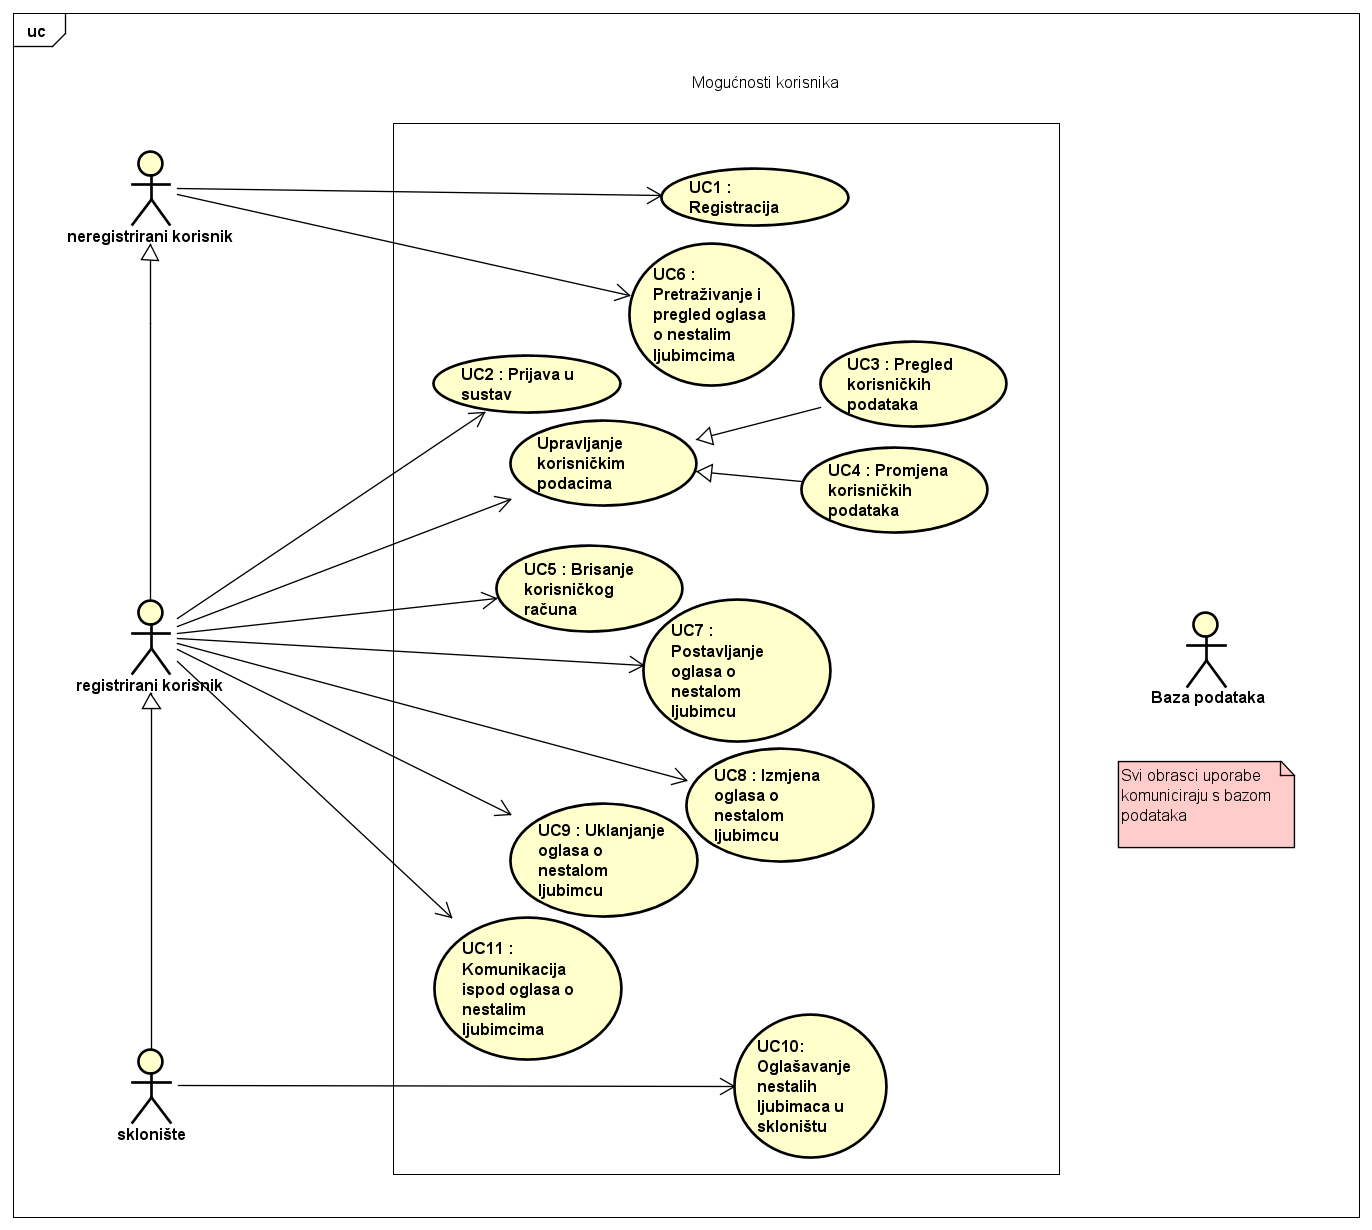
\includegraphics[scale=0.45]{slike/uc_mogucnosti_korisnika.PNG} 
					\centering
					\caption{Dijagram mogućnosti korisnika}
					\label{uc_mogucnosti_korisnika}
				\end{figure}
				
			\subsection{Sekvencijski dijagrami}
				
				\iffalse
				\textit{Nacrtati sekvencijske dijagrame koji modeliraju najvažnije dijelove sustava (max. 4 dijagrama). Ukoliko postoji nedoumica oko odabira, razjasniti s asistentom. Uz svaki dijagram napisati detaljni opis dijagrama.}
				\eject
				\fi
				
			\begin{figure}[H]
				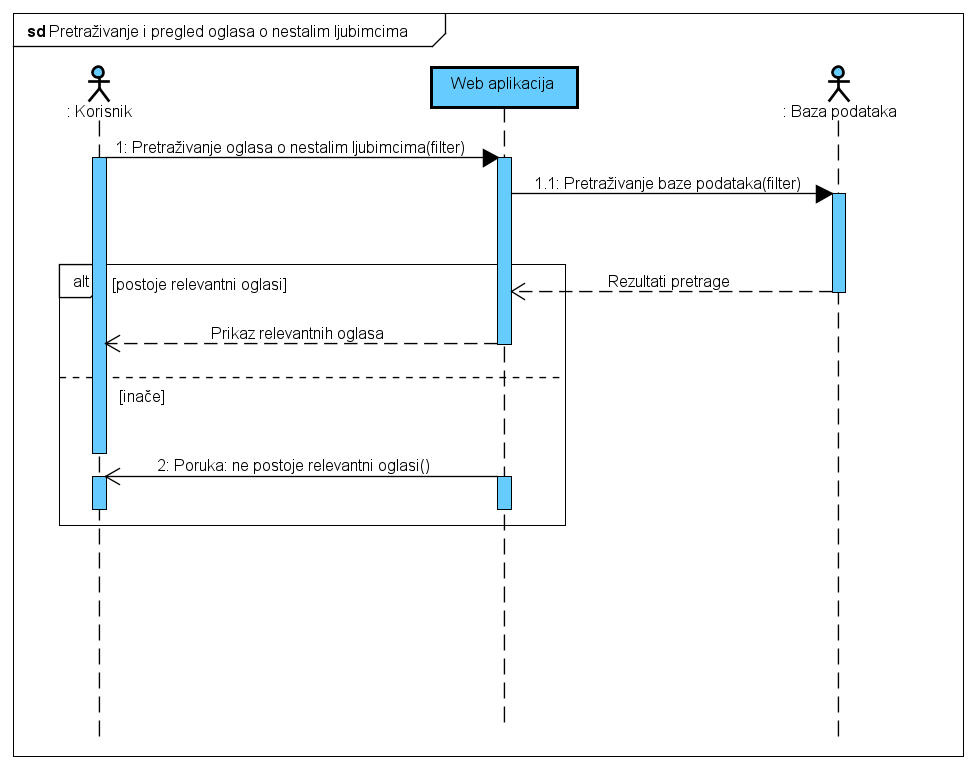
\includegraphics[scale=0.6]{slike/seq_pretrazivanje_pregled_oglasa.PNG} 
				\centering
				\caption{Sekvencijski dijagram pretraživanja i pregleda oglasa}
				\label{seq_pretrazivanje_pregled_oglasa}
			\end{figure}
			
			\noindent\textbf{Obrazac uporabe UC6 - Pretraživanje i pregled oglasa o nestalim ljubimcima}\newline
			\noindent Korisnik (neregistriran ili registriran) u tražilicu unosi podatke o životinji koja ga zanima. Filter tražilice ispunjava raznim vrijednostima po kojima se životinje razlikuju poput imena, vrste, lokacije nestanka, boji i vremenskom rasponu nestanka. Nakon toga se u bazi podataka traži podudarnost s traženim upitom i vraća se rezultat korisniku ovisno o nađenom. Korisniku će se prikazati relevantni oglasi ili (u slučaju da nema nikakvih podudarnosti) poruka da nema rezultata.
			
			
			\begin{figure}[H]
				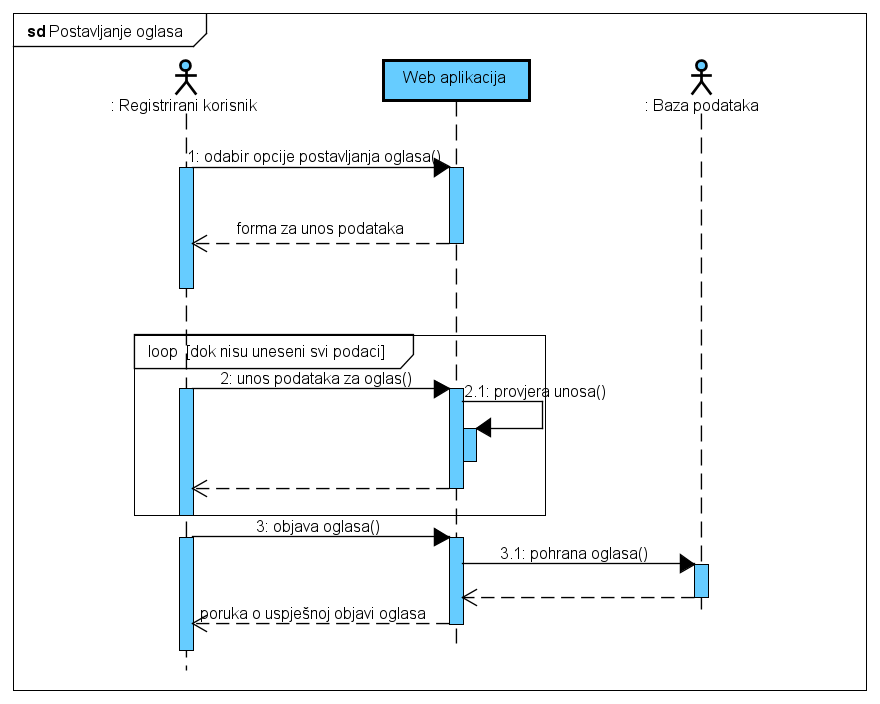
\includegraphics[scale=0.6]{slike/seq_postavljanje_oglasa.PNG} 
				\centering
				\caption{Sekvencijski dijagram postavljanja oglasa}
				\label{seq_postavljanje_oglasa}
			\end{figure}
			
			\noindent\textbf{Obrazac uporabe UC7 - Postavljanje oglasa o nestalom ljubimcu}\newline
			\noindent Korisnik nakon registracije i/ili prijave u sustav, ima, između ostalog, i mogućnost postavljanja oglasa. Korisnik na web stranici odabire opciju postavljanja oglasa čime mu se otvara forma za unos podataka kao što su vrsta, ime na koje se životinja odaziva, datum i sat nestanka, lokacija nestanka, boja, starost, tekstni opis pa čak i do 3 fotografije nestalog ljubimca. Ako korisnik nije unio sve potrebne podatke u aplikaciju za prijavu nestale životinje, sustav ga o tome obavještava i navodi na dio forme koji treba biti popunjen. Također, u slučaju da je registrirani korisnik sklonište za životinje, početna postavka kategorije oglasa je "U skloništu", a inače "Za ljubimcem se traga". Kad je korisnik spreman objaviti oglas mora stisnuti gumb "Objavi". Nakon što je stisnuo gumb za objavu, oglas se pohranjuje u bazu podataka, a korisniku pristiže poruka o uspješnom postavljanju oglasa.		
			
			\begin{figure}[H]
				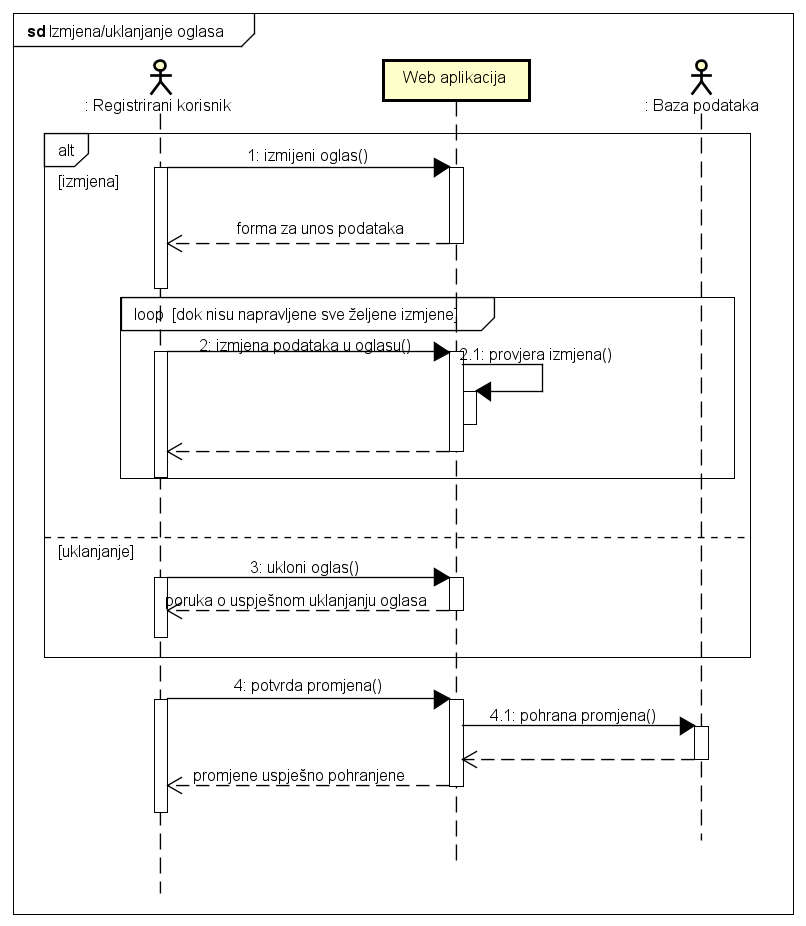
\includegraphics[scale=0.6]{slike/seq_izmjena_oglasa.PNG} 
				\centering
				\caption{Sekvencijski dijagram izmjenjivanja/brisanja oglasa}
				\label{seq_izmjena_oglasa}
			\end{figure}
			
			\noindent\textbf{Obrasci uporabe UC8 i UC9 - izmjena/uklanjanje oglasa o nestalom ljubimcu}\newline
			\noindent Nakon što je objavio oglas, registrirani korisnik može upravljati oglasom – raditi izmjene na njemu ili ga ukloniti. \\
Ako registrirani korisnik odabere opciju izmjene oglasa otvara mu se forma za izmjenu podataka. Korisnik može mijenjati određene podatke, a može promijeniti i kategoriju oglasa iz "Za ljubimcem se traga" u "Ljubimac je sretno pronađen", "Ljubimac nije pronađen, ali se za njim više aktivno ne traga" i "Ljubimac je pronađen uz nesretne okolnosti". Sustav nakon toga provjerava jesu li promijenjeni podaci adekvatni te šalje korisniku povratnu informaciju. \\

Ako korisnik odabere opciju za uklanjanje oglasa, sustav ga obavještava o uspješnom uklanjanju oglasa.\\
Nakon bilo koje od ovih radnji, korisnik potvrđuje promjenu u sustavu te se promjena pohranjuje u bazu podataka. Korisnik na kraju dobiva poruku kako je uspio izvršiti radnju.

	
		\section{Ostali zahtjevi}
		 
			 \begin{packed_item}
			 
			 \item Sustav treba omogućiti rad više korisnika u stvarnom vremenu
			 \item Sustav treba funkcionirati ispravno neovisno o web pregledniku ili uređaju
			 \item Korisničko sučelje i sustav moraju podržavati hrvatsku abecedu (dijakritičke znakove) pri unosu i prikazu tekstualnog sadržaja
			 \item Učitavanje početne stranice ne smije trajati duže od nekoliko sekundi
			 \item Izvršavanje dijela programa u kojem se pristupa bazi podataka ne smije trajati duže od nekoliko sekundi
			 \item Sustav treba biti implementiran kao (responzivna) web aplikacija koristeći objektno-orijentirane jezike
			 \item Neispravno korištenje korisničkog sučelja ne smije narušiti funkcionalnost i rad sustava
			 \item Nadogradnja sustava ne smije narušavati postojeće funkcionalnosti sustava
			 \item Sustav treba biti jednostavan za korištenje, korisnici se moraju znati koristiti sučeljem bez opširnih uputa
			 \item Veza s bazom mora biti kvalitetno zaštićena, brza i otporna na vanjske greške
			 \item Pristup sustavu mora biti omogućen iz javne mreže pomoću HTTPS
			 
			 
			 \end{packed_item}
			 
			 
			 
	
	\chapter{Arhitektura i dizajn sustava}
		
		Arhitektura se može podijeliti na 4 podsustava:
		\begin{packed_item}
		
			\item   Web poslužitelj
			\item   \textit{Front-end}
			\item 	\textit{Back-end}
			\item   Baza podataka
		\end{packed_item}
		
		
		\textit{Web poslužitelj} je program koji omogućuje korisnicima pristupanje internet resursima putem zahtjeva poslanih poslužiteljima. Web preglednik je prevoditelj koji web stranicu
pisanu u kodu interpretira i prikazuje u klijentu razumljivom obliku. Koristeći web preglednik
klijent šalje zahtjeve web poslužitelju.
		
		\textit{Front-end} web aplikacija omogućuje korisniku interakciju s \textit{back-end}-om na poslužitelju, koje se omogućuje kroz korisničko sučelje. 
		\textit{Front-end} aplikacija šalje zahtjeve \textit{back-end} aplikaciji koja ima ulogu web poslužitelja. Njezin je osnovni zadatak pohrana, obrada i dostava web stranica klijentu te nam ona predstavlja
centar za razmjenu informacija i pružanje usluga. Sam poslužitelj pokreće web aplikaciju i
prosljeđuje joj klijentske zahtjeve.\\

		Prednosti odabrane arhitekture su te što se slojevi mogu oblikovati odvojeno te sve
komponente mogu biti jednostavnije i razumljivije, ostvaruje se podjela brige (\textit{separation of
concerns}) time što svaki sloj brine o svojoj funkcionalnosti i ne miješa se u brige nekog
drugog sloja, a njihova međuovisnost ostvaruje se komunikacijom putem sučelja čija se
implementacija može prilagoditi u određenom sloju.\\

		\pagebreak

		\subsection{MVC stil arhitekture}
		Arhitektura	je	detaljnije	razrađena	najsličnija	stilu	arhitekture	MVC	(Model-view-controller).\\
		
		Osnovna	karakteristika ovog stila je	nezavisan razvoj	pojedinih dijelova aplikacije što omogućuje jednostavnije testiranje	i razvijanje dijelova sustava te	njihove	dorade.	
Korisničko	sučelje	je	odvojeno od	ostatka	sustava, a kohezija	elemenata se	postiže	kroz	
tri	sloja, jednog sloja	na klijentskoj strani - pogled (\textit{View}) te dva na	poslužiteljskoj	strani	
– upravitelj	(\textit{Controller})	i	model	(\textit{Model}).

		\begin{packed_enum}
			\item\textit{Model} - predstavlja glavnu komponentu sustava koja sadrži dinamičke strukture podataka odnosno razrede koji opisuju domenu primjene te sadrže pravila i aplikacijsku logiku. Blisko je povezan s bazom podataka aplikacije.
			\item\textit{Pogled (View)} - komponenta koja sadrži niz drugih komponenata koje služe za prikaz podataka modela i interakciju s korisnikom kroz grafičko sučelje.
			\item\textit{Upravitelj (Controller)} - komponenta koja upravlja korisničkim zahtjevima prema modelu i odgovorima modela natrag prema pogledima. Omogućuje poveznicu korisničke strane	s poslužiteljskom.
		\end{packed_enum}

		%unos slike
		\begin{figure}[H]
			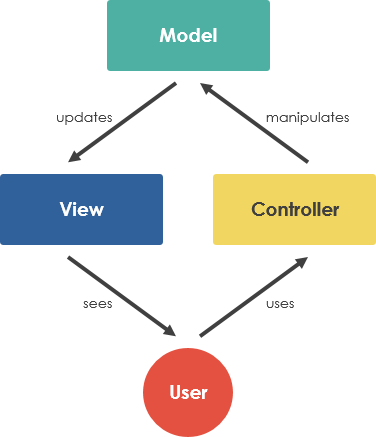
\includegraphics[scale=0.7]{slike/mvc-framework.PNG} 
			\centering
			\caption{MVC stil arhitekture}
			\label{mvc-framework}
		\end{figure}
	
		
		\section{Programski jezici, razvojni okviri, alati i biblioteke koda}
		
		
		\subsection{Back-end i baza podataka}
		U okviru \textit{back-end} aplikacije koriste se različiti alati i tehnologije kako bi se postigla funkcionalnost web aplikacije. 
		
		Sama funkcionalnost \textit{back-enda} ostvarena je koristeći \textit{Kotlin} i \textit{Spring Boot}, popularne \textit{frameworke} za Javu i Kotlin.
		
		\textit{Spring Boot} olakšava izradu web aplikacije pružajući razne automatske konfiguracije. To uvelike omogućava integraciju različitih dijelova aplikacije i pruža mnogo gotovih implementacija koje se koriste putem vrlo intuitivnih sučelja.
		
		Baza podataka ostvarena je u \textit{PostgreSQL}-u, a za njenu jasnu definiciju korišten je alat \textit{Flyway}. \textit{Flyway} omogućava precizno i upravljivo definiranje strukture baze podataka.
		
		Za preslikavanje entiteta iz \textit{PostgreSQL} baze podataka na klase u \textit{back-end} aplikaciji korišten je \textit{JPA (Jakarta Persistence API)}, koji značajno olakšava generiranje upita ovisno o pozivima metoda nad klasama entiteta, a za komunikaciju baze i same aplikacije koristi se \textit{JDBC (Java Database Connectivity)}.
		
		Za konfiguracijske datoteke aplikacije koristi se \textit{YAML} format. Upravljanje bazom podataka odvija se preko \textit{Datagrip}-a, a razvoj kompletne \textit{back-end} aplikacije obavlja se u \textit{IntelliJ IDEA}, popularnom alatu tvrtke \textit{JetBrains}. 
		
		Za izgradnju cijele aplikacije koristi se \textit{Gradle}, alat za automatizaciju izgradnje. 
\textit{JWT (JSON Web Token}) standard korišten je za sigurnost aplikacije, generirajući tokene, koji istovremeno služe za autorizaciju i autentifikaciju korisnika.


			\subsection{Front-end}
			U izradi \textit{front-end} dijela aplikacije koristimo niz tehnologija kako bismo postigli željene funkcionalnosti i estetski privlačan dizajn. Ključne tehnologije koje se koriste u razvoju uključuju \textit{TypeScript}, \textit{React}, \textit{Bootstrap}, \textit{Vite} i \textit{IntelliJ}.
			
\textit{React}, kao glavni okvir, omogućava olakšanu izradu web stranica i pruža širok spektar alata za navigaciju, dohvaćanje i prikazivanje podataka. Koristi se označni kod sličan \textit{HTML}-u, obogaćen mogućnostima \textit{TypeScript}-a za definiranje sadržaja stranica, dok se za definiranje stila i izgleda koristi \textit{Bootstrap}.

Za efikasno upravljanje podacima u aplikaciji koristi se \textit{React Query}. \textit{Vite}, alat za brzu izgradnju aplikacija, osigurava optimiziran razvojni proces i ubrzanje vremena učitavanja stranica.

Konačno, za pisanje \textit{TypeScript} koda koristi se \textit{IntelliJ}, moćno razvojno okruženje koje omogućava precizno kodiranje i upravljanje projektom. Ovaj skup tehnologija omogućava nam izradu kvalitetne \textit{front-end} aplikacije s visokom funkcionalnošću i atraktivnim dizajnom.\\
		
		
				
		\section{Baza podataka}
			
		

			\subsection{Opis tablica}
			

				\textbf{APP\_USER} Predstavlja registriranog korisnika aplikacije, u \textit{@ManyToOne} vezi s \textbf{USER\_TYPE} preko \textit{userTypeId}.
				
				
				\begin{longtblr}[
					label=none,
					entry=none
					]{
						width = \textwidth,
						colspec={|X[8,l]|X[6, l]|X[18, l]|}, 
						rowhead = 1,
					} %definicija širine tablice, širine stupaca, poravnanje i broja redaka naslova tablice
					\hline \SetCell[c=3]{c}{\textbf{APP\_USER}}	 \\ \hline[3pt]
					\SetCell{LightGreen}userId & BIGINT	&  	jedinstveni ID korisnika  	\\ \hline
					username	& VARCHAR &   korisničko ime (jedinstveno)	\\ \hline 
					email & VARCHAR &   korisnikova e-mail adresa (jedinstvena)	\\ \hline 
					password & VARCHAR	&  	korisnikova lozinka	\\ \hline 
					name & VARCHAR	&  	ime korisnika	\\ \hline 
					telephone\_number & VARCHAR	&  	korisnikov broj telefona (jedinstven)	\\ \hline 
					\SetCell{LightBlue} userTypeId	& BIGINT &   ID koji označava tip korisnika	\\ \hline 
				\end{longtblr}
				
				\noindent\textbf{USER\_TYPE} Predstavlja popis tipova korisnika aplikacije (userTypeId=1 odgovara osobi, userTypeId=2 skloništu).
				
				
				\begin{longtblr}[
					label=none,
					entry=none
					]{
						width = \textwidth,
						colspec={|X[8,l]|X[6, l]|X[18, l]|}, 
						rowhead = 1,
					} %definicija širine tablice, širine stupaca, poravnanje i broja redaka naslova tablice
					\hline \SetCell[c=3]{c}{\textbf{USER\_TYPE}}	 \\ \hline[3pt]
					\SetCell{LightGreen}userTypeId & BIGINT	&  	jedinstveni ID tipa korisnika  	\\ \hline
					name	& VARCHAR &   ime tipa korisnika	\\ \hline 
				\end{longtblr}
				
				\noindent\textbf{MESSAGE} Poruka koju korisnici mogu ostavljati u komunikaciji ispod oglasa, u \textit{@ManyToOne} vezi s \textbf{AD} preko \textit{adId}, \textit{@ManyToOne} vezi s \textbf{USER} preko \textit{userId}, \textit{@OneToOne} vezi s \textbf{IMAGE} preko \textit{imageId}.
				
				\begin{longtblr}[
					label=none,
					entry=none
					]{
						width = \textwidth,
						colspec={|X[8,l]|X[6, l]|X[18, l]|}, 
						rowhead = 1,
					} %definicija širine tablice, širine stupaca, poravnanje i broja redaka naslova tablice
					\hline \SetCell[c=3]{c}{\textbf{MESSAGE}}	 \\ \hline[3pt]
					\SetCell{LightGreen}messageId & BIGINT	&  	jedinstveni ID poruke  	\\ \hline
					text	& VARCHAR &   sadržaj poruke	\\ \hline 
					date	& DATE &   datum kada je poruka ostavljena ispod oglasa	\\ \hline 
					latitude	& DOUBLE PRECISION &   geografska širina s koje je poruka ostavljena	\\ \hline 
					longitude	& DOUBLE PRECISION &   geografska dužina s koje je poruka ostavljena	\\ \hline 
					\SetCell{LightBlue}adId	& BIGINT &   jedinstveni ID oglasa ispod kojeg je poruka ostavljena	\\ \hline 
					\SetCell{LightBlue}userId	& BIGINT &   jedinstveni ID korisnika koji je ostavio poruku	\\ \hline 
					\SetCell{LightBlue}imageId	& BIGINT &   jedinstveni ID slike ostavljene uz poruku	\\ \hline 
					\SetCell{LightBlue}cityId	& BIGINT &   jedinstveni ID grada u kojem je poruka ostavljena	\\ \hline 
				\end{longtblr}
				
				\noindent\textbf{IMAGE} Tablica u koju se spremaju slike koje se dohvaćaju preko URL.
				
				\begin{longtblr}[
					label=none,
					entry=none
					]{
						width = \textwidth,
						colspec={|X[8,l]|X[6, l]|X[18, l]|}, 
						rowhead = 1,
					} %definicija širine tablice, širine stupaca, poravnanje i broja redaka naslova tablice
					\hline \SetCell[c=3]{c}{\textbf{IMAGE}}	 \\ \hline[3pt]
					\SetCell{LightGreen}imageId & BIGINT	&  	jedinstveni ID slike  	\\ \hline
					imageUrl	& VARCHAR &   URL slike	\\ \hline 
				\end{longtblr}
				
				\noindent\textbf{ACTIVITY} Predstavlja kategoriju oglasa.
				
				\begin{longtblr}[
					label=none,
					entry=none
					]{
						width = \textwidth,
						colspec={|X[8,l]|X[6, l]|X[18, l]|}, 
						rowhead = 1,
					} %definicija širine tablice, širine stupaca, poravnanje i broja redaka naslova tablice
					\hline \SetCell[c=3]{c}{\textbf{ACTIVITY}}	 \\ \hline[3pt]
					\SetCell{LightGreen}activityId & BIGINT	&  	jedinstveni ID kategorije  	\\ \hline
					activityCategory	& VARCHAR &   naziv kategorije	\\ \hline 
				\end{longtblr}
				
				\noindent\textbf{AD} Predstavlja oglas, u \textit{@ManyToOne} vezi s \textbf{ACTIVITY}, \textit{@ManyToOne} vezi s \textbf{USER} preko \textit{userId}, \textit{@OneToOne} vezi s \textbf{IMAGE} (moguće 3 slike po oglasu), \textit{@OneToOne} vezi s \textbf{PET}.
				
				\begin{longtblr}[
					label=none,
					entry=none
					]{
						width = \textwidth,
						colspec={|X[8,l]|X[6, l]|X[18, l]|}, 
						rowhead = 1,
					} %definicija širine tablice, širine stupaca, poravnanje i broja redaka naslova tablice
					\hline \SetCell[c=3]{c}{\textbf{AD}}	 \\ \hline[3pt]
					\SetCell{LightGreen}adId & BIGINT	&  	jedinstveni ID oglasa  	\\ \hline
					inShelter	& INT &   1 ako je oglas od skloništa, inače 0 	\\ \hline 
					\SetCell{LightBlue}userId	& BIGINT &   jedinstveni ID korisnika koji je postavio oglas 	\\ \hline 
					\SetCell{LightBlue}activityId	& BIGINT &   jedinstveni ID kategorije oglasa 	\\ \hline
					\SetCell{LightBlue}image1Id	& BIGINT &   jedinstveni ID prve slike 	\\ \hline
					\SetCell{LightBlue}image2Id	& BIGINT &   jedinstveni ID druge slike 	\\ \hline
					\SetCell{LightBlue}image3Id	& BIGINT &   jedinstveni ID treće slike 	\\ \hline
					\SetCell{LightBlue}petId	& BIGINT &   jedinstveni ID ljubimca u oglasu 	\\ \hline
				\end{longtblr}
				
				\noindent\textbf{PET} Predstavlja ljubimca, u \textit{@ManyToMany} vezi s \textbf{COLOR}, \textit{@ManyToOne} vezi sa \textbf{SPECIES}, \textit{@ManyToOne} vezi sa \textbf{CITY}.
				
				\begin{longtblr}[
					label=none,
					entry=none
					]{
						width = \textwidth,
						colspec={|X[8,l]|X[6, l]|X[18, l]|}, 
						rowhead = 1,
					} %definicija širine tablice, širine stupaca, poravnanje i broja redaka naslova tablice
					\hline \SetCell[c=3]{c}{\textbf{PET}}	 \\ \hline[3pt]
					\SetCell{LightGreen}petId & BIGINT	&  	jedinstveni ID ljubimca  	\\ \hline
					hourMissing	& INT &   sat nestanka ljubimca	\\ \hline 
					dateMissing	& DATE &   datum nestanka ljubimca	\\ \hline 
					age	& INT &   starost ljubimca	\\ \hline 
					description	& VARCHAR &   opis ljubimca	\\ \hline 
					latitude	& DOUBLE PRECISION &   geografska širina lokacije ljubimca	\\ \hline 
					longitude	& DOUBLE PRECISION &   geografska dužina lokacije ljubimca	\\ \hline 
					petName	& VARCHAR &   ime na koje se ljubimac odaziva	\\ \hline 
					\SetCell{LightBlue}speciesId	& BIGINT &   jedinstveni ID vrste ljubimca	\\ \hline 
					\SetCell{LightBlue}cityId	& BIGINT &   jedinstveni ID grada	\\ \hline 
				\end{longtblr}
				
				\noindent\textbf{SPECIES} Tablica vrsta ljubimaca.
				
				\begin{longtblr}[
					label=none,
					entry=none
					]{
						width = \textwidth,
						colspec={|X[8,l]|X[6, l]|X[18, l]|}, 
						rowhead = 1,
					} %definicija širine tablice, širine stupaca, poravnanje i broja redaka naslova tablice
					\hline \SetCell[c=3]{c}{\textbf{SPECIES}}	 \\ \hline[3pt]
					\SetCell{LightGreen}speciesId & BIGINT	&  	jedinstveni ID vrste ljubimca  	\\ \hline
					speciesName	& VARCHAR &   naziv vrste ljubimca	\\ \hline 
				\end{longtblr}
				
				\noindent\textbf{COLOR} Tablica s bojama ljubimaca, u \textit{@ManyToMany} vezi s \textbf{PET}.
				
				\begin{longtblr}[
					label=none,
					entry=none
					]{
						width = \textwidth,
						colspec={|X[8,l]|X[6, l]|X[18, l]|}, 
						rowhead = 1,
					} %definicija širine tablice, širine stupaca, poravnanje i broja redaka naslova tablice
					\hline \SetCell[c=3]{c}{\textbf{COLOR}}	 \\ \hline[3pt]
					\SetCell{LightGreen}colorId & BIGINT	&  	jedinstveni ID boje  	\\ \hline
					colorName	& VARCHAR &   naziv boje	\\ \hline 
				\end{longtblr}
				
				\noindent\textbf{OF\_COLOR} Tablica veze između \textbf{PET} i \textbf{COLOR}.
				
				\begin{longtblr}[
					label=none,
					entry=none
					]{
						width = \textwidth,
						colspec={|X[8,l]|X[6, l]|X[18, l]|}, 
						rowhead = 1,
					} %definicija širine tablice, širine stupaca, poravnanje i broja redaka naslova tablice
					\hline \SetCell[c=3]{c}{\textbf{OF\_COLOR}}	 \\ \hline[3pt]
					\SetCell{LightBlue}colorId & BIGINT	&  	jedinstveni ID boje  	\\ \hline
					\SetCell{LightBlue}petId & BIGINT	&  	jedinstveni ID ljubimca	\\ \hline
				\end{longtblr}
				
				\noindent\textbf{COUNTY} Predstavlja županije nestanka/pronalaska ljubimaca.
				
				\begin{longtblr}[
					label=none,
					entry=none
					]{
						width = \textwidth,
						colspec={|X[8,l]|X[6, l]|X[18, l]|}, 
						rowhead = 1,
					} %definicija širine tablice, širine stupaca, poravnanje i broja redaka naslova tablice
					\hline \SetCell[c=3]{c}{\textbf{COUNTY}}	 \\ \hline[3pt]
					\SetCell{LightGreen}countyId & BIGINT	&  	jedinstveni ID županije  	\\ \hline
					countyName & VARCHAR	&  	naziv županije	\\ \hline
				\end{longtblr}
				
				\noindent\textbf{CITY} Predstavlja gradove nestanka/pronalaska ljubimaca, u \textit{@ManyToOne} vezi s \textbf{COUNTY}.
				
				\begin{longtblr}[
					label=none,
					entry=none
					]{
						width = \textwidth,
						colspec={|X[8,l]|X[6, l]|X[18, l]|}, 
						rowhead = 1,
					} %definicija širine tablice, širine stupaca, poravnanje i broja redaka naslova tablice
					\hline \SetCell[c=3]{c}{\textbf{CITY}}	 \\ \hline[3pt]
					\SetCell{LightGreen}cityId & BIGINT	&  	jedinstveni ID grada  	\\ \hline
					cityName & VARCHAR	&  	naziv grada	\\ \hline
					\SetCell{LightBlue}countyId & BIGINT	&  	jedinstveni ID županije  	\\ \hline
					
				\end{longtblr}
				
			
			\subsection{Dijagram baze podataka}
			\begin{figure}[H]
				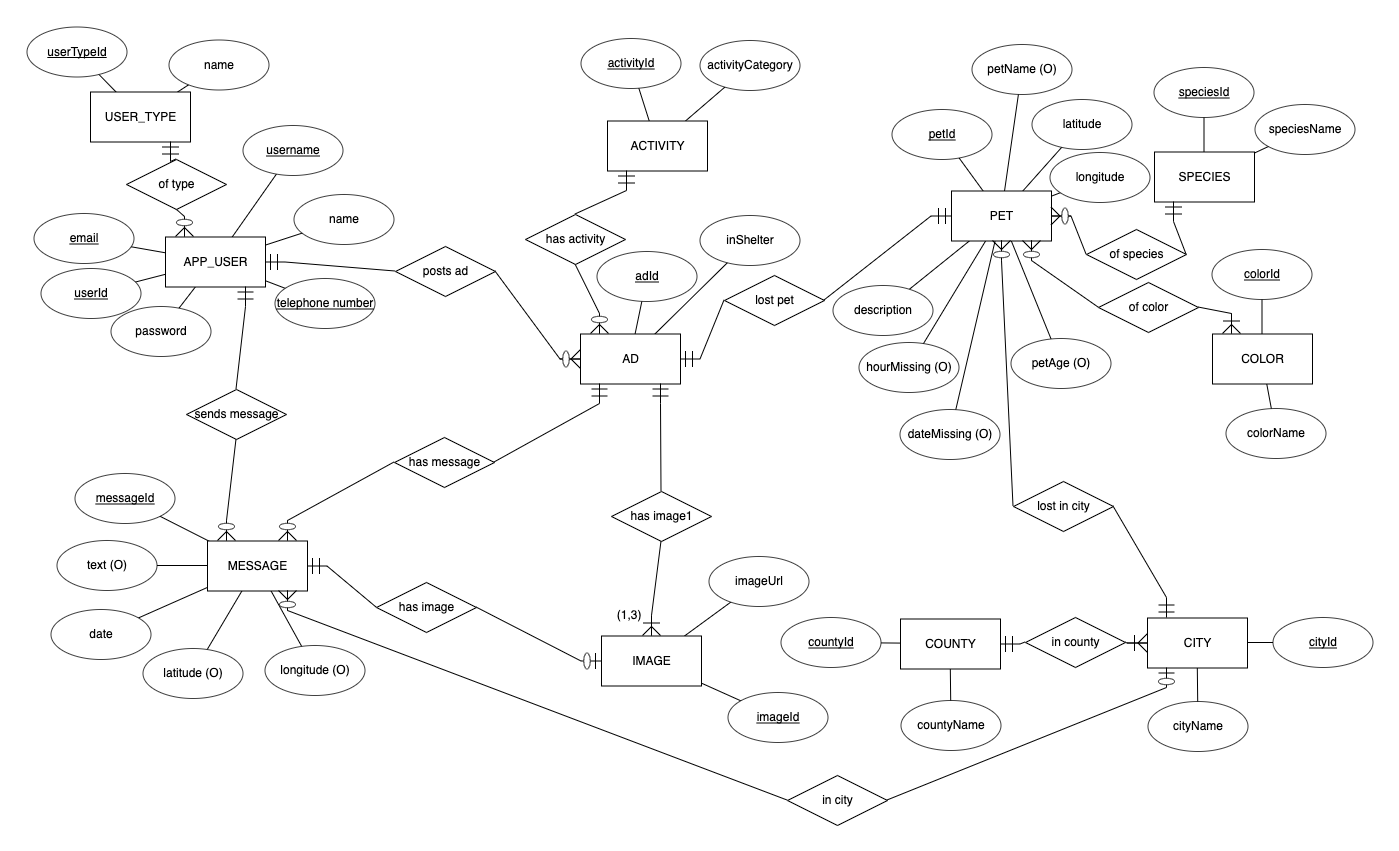
\includegraphics[scale=0.33]{slike/ER_diagram.PNG} 
				\centering
				\caption{ER dijagram baze podataka}
				\label{ER_diagram}
			\end{figure}
			
			\begin{figure}[H]
				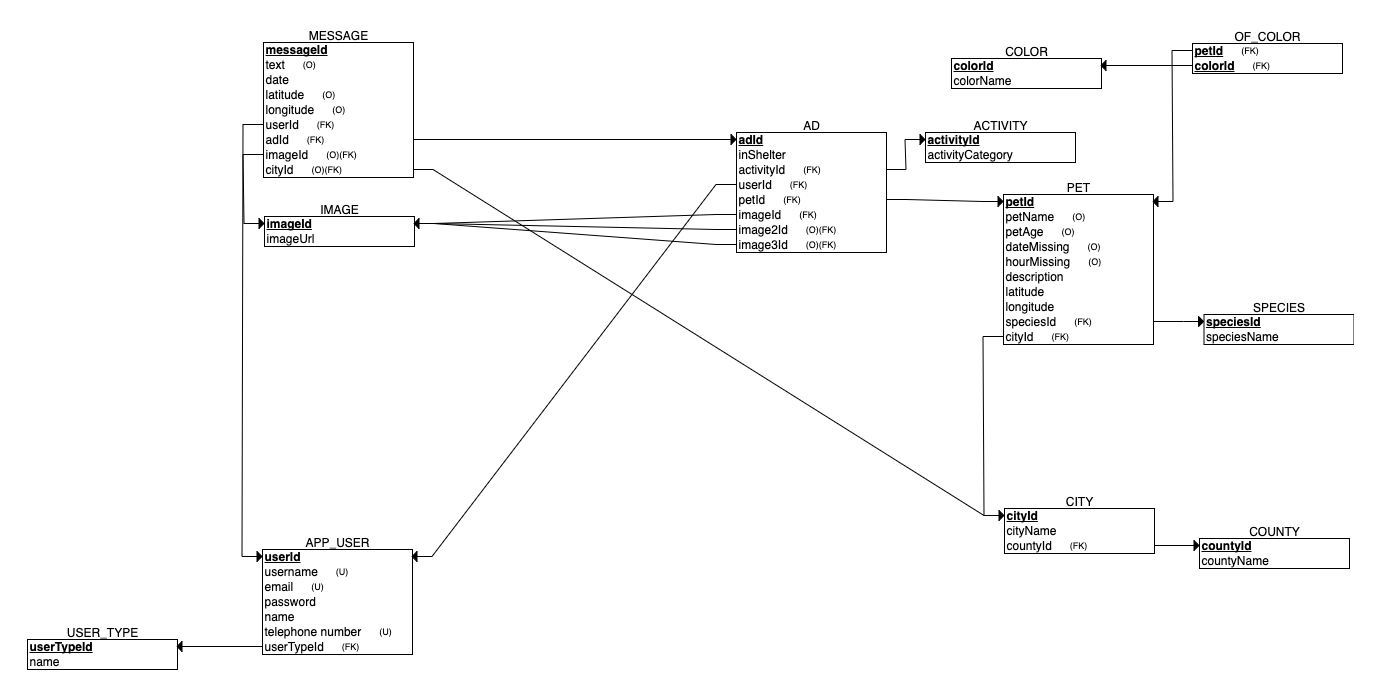
\includegraphics[scale=0.34]{slike/relational_diagram.PNG} 
				\centering
				\caption{Relacijski dijagram baze podataka}
				\label{relational_diagram}
			\end{figure}
			
			\eject
			
			
		\section{Dijagram razreda}
		
			\textit{Potrebno je priložiti dijagram razreda s pripadajućim opisom. Zbog preglednosti je moguće dijagram razlomiti na više njih, ali moraju biti grupirani prema sličnim razinama apstrakcije i srodnim funkcionalnostima.}\\
			
			\textbf{\textit{dio 1. revizije}}\\
			
			\textit{Prilikom prve predaje projekta, potrebno je priložiti potpuno razrađen dijagram razreda vezan uz \textbf{generičku funkcionalnost} sustava. Ostale funkcionalnosti trebaju biti idejno razrađene u dijagramu sa sljedećim komponentama: nazivi razreda, nazivi metoda i vrste pristupa metodama (npr. javni, zaštićeni), nazivi atributa razreda, veze i odnosi između razreda.}\\
			
			\iffalse
			\textbf{\textit{dio 2. revizije}}\\			
			
			\textit{Prilikom druge predaje projekta dijagram razreda i opisi moraju odgovarati stvarnom stanju implementacije}
			\fi
			
			
			\eject
		
		\iffalse
		\section{Dijagram stanja}
			
			
			\textbf{\textit{dio 2. revizije}}\\
			
			\textit{Potrebno je priložiti dijagram stanja i opisati ga. Dovoljan je jedan dijagram stanja koji prikazuje \textbf{značajan dio funkcionalnosti} sustava. Na primjer, stanja korisničkog sučelja i tijek korištenja neke ključne funkcionalnosti jesu značajan dio sustava, a registracija i prijava nisu. }
			
			
			\eject 
		\fi		
		
		\iffalse
		\section{Dijagram aktivnosti}
			
			\textbf{\textit{dio 2. revizije}}\\
			
			 \textit{Potrebno je priložiti dijagram aktivnosti s pripadajućim opisom. Dijagram aktivnosti treba prikazivati značajan dio sustava.}
			
			\eject
		\fi
		
		\iffalse
		\section{Dijagram komponenti}
		
			\textbf{\textit{dio 2. revizije}}\\
		
			 \textit{Potrebno je priložiti dijagram komponenti s pripadajućim opisom. Dijagram komponenti treba prikazivati strukturu cijele aplikacije.}
		\fi
	\chapter{Implementacija i korisničko sučelje}
		
		
		\section{Korištene tehnologije i alati}
		
			Komunikacija u timu ostvarena je pomoću $Discord^{1}$ platforme koja nudi opcije tekstualnog dopisivanja, glasovnog poziva i video-chat-a. U serveru našeg projektnog tima postojalo je nekoliko kanala koji su se bavili različitim temama (back-end, front-end, dokumentacija…) što nam je pomoglo u podjeli posla i filtriranju zadataka. Za izradu UML dijagrama koristili smo se aplikacijom $Astah^{2}$ pomoću koje smo vrlo jednostavno napravili željene dijagrame i time pokazali ideju projektnog zadatka, kao i način rada naše aplikacije. Udaljeni repozitorij projekta dostupan je na web platformi $GitHub^{3}$.\\
Za razvojno okruženje koristili smo $Visual Studio Code (VSC)^{4}$ i $IntelliJ IDEA^{5}$. VSC nudi široku podršku za jezike i ekstenzije, integraciju s Git-om i različitim alatima i servisima ($Docker^{6}$) te snimanje koraka za debugging. Također, dolazi s ugrađenom podrškom za $JavaScript^{7}$ i $TypeScript^{8}$. IntelliJ IDEA smatra se dobrim izborom IDE-a jer nudi programeru naprednu podršku za pisanje koda (Code Assistance), odličan debugger, refaktoriranje koda te podršku za različite tehnologije (Spring Framework, JavaScript, HTML, CSS, TypeScript, React, SQL) i jezike (Java, Kotlin, Groovy). \\
Klijentska strana aplikacije (\textit{front-end}) napisana je $React^{9}$-om preko TypeScript-a i $Vite.js^{10}$-om. $Material UI^{11}$ je biblioteka React komponenata koja pruža implementaciju Google-ovog Material Design koncepta u React aplikacijama, a fokusiran je na stvaranje dosljednih i intuitivnih korisničkih sučelja.\\
Poslužiteljska strana aplikacije (\textit{back-end}) napisana je $Kotlin^{12}$-om i $Spring Framework^{13}$-om. Kotlin omogućuje interoperabilnost s jezikom $Java^{14}$ (može se koristiti zajedno s njim u sklopu istog projekta te koristiti njegove biblioteke). Spring Framework je open-source radni okvir za razvoj aplikacija baziranih na Javi. On implementira inverziju kontrole (IoC), uvođenje ovisnosti (DI), Model-View-Controller (MVC), pristup podacima, sigurnost i Spring Boot.\\
Pokretanje, izvršavanje i puštanje u pogon izvršavaju se preko 3 kontejnera platforme Docker koji pokrivaju najvažnije dijelove aplikacije: back-end, front-end i PostgreSQL bazu podataka. Pri deployment-u projekta koristimo radni okvir $Express.js^{15}$ za izgradnju API-ja s $Node.js^{16}$ radnim okruženjem.\\


\begin{footnotesize}
	\noindent $^1$\href{https://discord.com/}{https://discord.com/} \\
	$^2$\href{https://astah.net/}{https://astah.net/} \\
	$^3$\href{https://github.com/}{https://github.com/} \\
	$^4$\href{https://code.visualstudio.com/}{https://code.visualstudio.com/} \\
	$^5$\href{https://www.jetbrains.com/idea/}{https://www.jetbrains.com/idea/} \\
	$^6$\href{https://www.docker.com/}{https://www.docker.com/} \\
	$^7$\href{https://www.javascript.com/}{https://www.javascript.com/} \\
	$^8$\href{https://www.typescriptlang.org/}{https://www.typescriptlang.org/} \\
	$^9$\href{https://react.dev/}{https://react.dev/} \\
	$^{10}$\href{https://vitejs.dev/}{https://vitejs.dev/} \\
	$^{11}$\href{https://mui.com/}{https://mui.com/} \\
	$^{12}$\href{https://kotlinlang.org/}{https://kotlinlang.org/} \\
	$^{13}$\href{https://spring.io/projects/spring-framework/}{https://spring.io/projects/spring-framework/} \\
	$^{14}$\href{https://www.java.com/en/}{https://www.java.com/en/} \\
	$^{15}$\href{https://expressjs.com/}{https://expressjs.com/} \\
	$^{16}$\href{https://nodejs.org/en}{https://nodejs.org/en}
\end{footnotesize}
			
			
			\eject 
		
	
		\section{Ispitivanje programskog rješenja}
			
			\textbf{\textit{dio 2. revizije}}\\
			
			 \textit{U ovom poglavlju je potrebno opisati provedbu ispitivanja implementiranih funkcionalnosti na razini komponenti i na razini cijelog sustava s prikazom odabranih ispitnih slučajeva. Studenti trebaju ispitati temeljnu funkcionalnost i rubne uvjete.}
	
			
			\subsection{Ispitivanje komponenti}
			\textit{Potrebno je provesti ispitivanje jedinica (engl. unit testing) nad razredima koji implementiraju temeljne funkcionalnosti. Razraditi \textbf{minimalno 6 ispitnih slučajeva} u kojima će se ispitati redovni slučajevi, rubni uvjeti te izazivanje pogreške (engl. exception throwing). Poželjno je stvoriti i ispitni slučaj koji koristi funkcionalnosti koje nisu implementirane. Potrebno je priložiti izvorni kôd svih ispitnih slučajeva te prikaz rezultata izvođenja ispita u razvojnom okruženju (prolaz/pad ispita). }
			
			
			
			\subsection{Ispitivanje sustava}
			
			 \textit{Potrebno je provesti i opisati ispitivanje sustava koristeći radni okvir Selenium\footnote{\url{https://www.seleniumhq.org/}}. Razraditi \textbf{minimalno 4 ispitna slučaja} u kojima će se ispitati redovni slučajevi, rubni uvjeti te poziv funkcionalnosti koja nije implementirana/izaziva pogrešku kako bi se vidjelo na koji način sustav reagira kada nešto nije u potpunosti ostvareno. Ispitni slučaj se treba sastojati od ulaza (npr. korisničko ime i lozinka), očekivanog izlaza ili rezultata, koraka ispitivanja i dobivenog izlaza ili rezultata.\\ }
			 
			 \textit{Izradu ispitnih slučajeva pomoću radnog okvira Selenium moguće je provesti pomoću jednog od sljedeća dva alata:}
			 \begin{itemize}
			 	\item \textit{dodatak za preglednik \textbf{Selenium IDE} - snimanje korisnikovih akcija radi automatskog ponavljanja ispita	}
			 	\item \textit{\textbf{Selenium WebDriver} - podrška za pisanje ispita u jezicima Java, C\#, PHP koristeći posebno programsko sučelje.}
			 \end{itemize}
		 	\textit{Detalji o korištenju alata Selenium bit će prikazani na posebnom predavanju tijekom semestra.}
			
			\eject 
		
		
		\section{Dijagram razmještaja}
			
			\textbf{\textit{dio 2. revizije}}
			
			 \textit{Potrebno je umetnuti \textbf{specifikacijski} dijagram razmještaja i opisati ga. Moguće je umjesto specifikacijskog dijagrama razmještaja umetnuti dijagram razmještaja instanci, pod uvjetom da taj dijagram bolje opisuje neki važniji dio sustava.}
			
			\eject 
		
		\section{Upute za puštanje u pogon}
		
			\textbf{\textit{dio 2. revizije}}\\
		
			 \textit{U ovom poglavlju potrebno je dati upute za puštanje u pogon (engl. deployment) ostvarene aplikacije. Na primjer, za web aplikacije, opisati postupak kojim se od izvornog kôda dolazi do potpuno postavljene baze podataka i poslužitelja koji odgovara na upite korisnika. Za mobilnu aplikaciju, postupak kojim se aplikacija izgradi, te postavi na neku od trgovina. Za stolnu (engl. desktop) aplikaciju, postupak kojim se aplikacija instalira na računalo. Ukoliko mobilne i stolne aplikacije komuniciraju s poslužiteljem i/ili bazom podataka, opisati i postupak njihovog postavljanja. Pri izradi uputa preporučuje se \textbf{naglasiti korake instalacije uporabom natuknica} te koristiti što je više moguće \textbf{slike ekrana} (engl. screenshots) kako bi upute bile jasne i jednostavne za slijediti.}
			
			
			 \textit{Dovršenu aplikaciju potrebno je pokrenuti na javno dostupnom poslužitelju. Studentima se preporuča korištenje neke od sljedećih besplatnih usluga: \href{https://aws.amazon.com/}{Amazon AWS}, \href{https://azure.microsoft.com/en-us/}{Microsoft Azure} ili \href{https://www.heroku.com/}{Heroku}. Mobilne aplikacije trebaju biti objavljene na F-Droid, Google Play ili Amazon App trgovini.}
			
			
			\eject 
	\chapter{Zaključak i budući rad}
		
		Zadatak naše grupe bio je napraviti web aplikaciju koja bi pomogla opet ujediniti vlasnike sa svojim nestalim ljubimcima. Aplikacija služi kao svojevrsni portal s oglasima o izgubljenim, ali i pronađenim životinjama.\\
		Aplikaciju smo izrađivali tijekom oba nastavna ciklusa predmeta što je trajalo otprilike 14 tjedana. U svakom ciklusu smo imali zadatke koje smo morali ispuniti do unaprijed zadanog roka, a na kraju svakog ciklusa se ocjenjivao naš rad i uspjeh projektnog zadatka.\\
		U prvoj reviziji projekta, naglasak je bio na dokumentaciji i na izradi temelja za programsku potporu naše web aplikacije. Na početku projekta znali smo da je važno imati dobru povezanost i komunikaciju unutar tima te je uslijedilo upoznavanje članova, podjela posla i rasprava o potencijalnim načinima i tehnologijama pomoću kojih bismo mogli provesti ovaj projekt. Posao smo podijelili po parovima za izradu klijentske i poslužiteljske strane aplikacije te izradu dokumentacije, a znalo se dogoditi i da si svi članovi međusobno pomažu čime smo ubrzali proces izrade aplikacije, ali i podijelili znanje. Krenuli smo izradom modela baze podataka i pisanjem dokumentacije, a kako smo se bližili kraju prve faze projekta krenuli smo i s implementacijom pojedinih obrazaca uporabe i povezivanjem klijentske i poslužiteljske strane. Ipak, izrada dokumentacije je imala glavnu riječ u ovoj fazi projekta. Shvatili smo da trebamo velik fokus staviti na dijagram baze podataka, smišljanje obrazaca uporabe, sekvencijskih dijagrama i dijagram razreda jer će upravo oni biti podloga za razvoj programske potpore naše aplikacije. Pomogli su nam da unaprijed uvidimo gdje bi mogli izviriti problemi i koji su dijelovi ključni za dobru izradu i izvedbu našeg portala.\\
		Za drugu reviziju naglasak se prebacio na samu implementaciju programske potpore za sve funkcionalnosti koje nisu uključene u izvedbu tijekom prve revizije. U ovom dijelu su članovi tima koji su radili \textit{back-end} puno više komunicirali s onima koji su radili \textit{front-end} jer su njihovi zadaci ovisili jedni od drugima. Dijagrami su u ovoj fazi prikazivali stanja objekata i njihove prijelaze, način funkcioniranja aplikacije (odnos između korisnika, web stranice i baze podataka) te organizaciju i međuovisnost komponenti.\\
		Očekivali smo da ćemo projekt uspješno svladati, iako su svi članovi imali različita iskustva i znanja. To se i dogodilo, a svaki je član ponešto novo naučio i upoznao se s tehnologijom koju je koristio pri rješavanju svog dijela projektnog zadatka. Naravno, svi su članovi međusobno dijelili sve što su do nekog trenutka naučili. Na početku su možda iskusniji članovi uzeli inicijativu u svoje ruke, ali s rastom projekta i novim naučenim znanjem drugi su ih članovi dostigli i svi su jednako doprinosili projektu. Članovi koji su se već bili susreli s potencijalnim problemima znali su kako reagirati i po mogućnosti ih izbjeći. Kada bi jedan član završio s nekim dijelom zadatka, drugi član/ovi bi pregledali zadovoljava li napravljeno sve što je i trebalo i time bismo skratili vrijeme izrade projekta jer bi moguća greška bila na vrijeme uočena.\\
		Komunikacija vezana uz projekt održana je preko Discord-a gdje su postojali kanali za različite dijelove projekta. Najčešće smo komunicirali preko poruka, a sastanci su se odvijali uživo i preko video-poziva. \\
		Sudjelovanjem u ovom projektu svi su članovi nešto novo naučili, čak i oni koji su imali nešto više znanja od drugih. Možemo reći da se svi ponešto odvažnije osjećamo po pitanju ovakvog tipa projektnog zadatka. Na kraju projekta smo shvatili što se sve od nas očekuje pri izradi web aplikacije te kako sve zahtjeve implementirati i povezati tako da sustav bude samoodrživ. Također smo shvatili da svaki član mora dati sve od sebe za dio zadatka kojeg radi, proučiti literaturu i istražiti nešto novo kako bismo probali izbjeći zaostatke i imali kontinuirani rast i razvoj web aplikacije.
		
		\eject 
	\chapter*{Popis literature}
		\addcontentsline{toc}{chapter}{Popis literature}
	 	
 		\textbf{\textit{Kontinuirano osvježavanje}}
	
		\textit{Popisati sve reference i literaturu koja je pomogla pri ostvarivanju projekta.}
		
		
		\begin{enumerate}
			
			
			\item  Programsko inženjerstvo, FER ZEMRIS, \url{http://www.fer.hr/predmet/proinz}
			
			\item  I. Sommerville, "Software engineering", 8th ed, Addison Wesley, 2007.
			
			\item  T.C.Lethbridge, R.Langaniere, "Object-Oriented Software Engineering", 2nd ed. McGraw-Hill, 2005.
			
			\item  I. Marsic, Software engineering book``, Department of Electrical and Computer Engineering, Rutgers University, \url{http://www.ece.rutgers.edu/~marsic/books/SE}
			
			\item  The Unified Modeling Language, \url{https://www.uml-diagrams.org/}
			
			\item  Astah Community, \url{http://astah.net/editions/uml-new}
		\end{enumerate}
		
		 
	
	
	\begingroup
	\renewcommand*\listfigurename{Indeks slika i dijagrama}
	%\renewcommand*\listtablename{Indeks tablica}
	%\let\clearpage\relax
	\listoffigures
	%\vspace{10mm}
	%\listoftables
	\endgroup
	\addcontentsline{toc}{chapter}{Indeks slika i dijagrama}


	
	\eject 
		
	\chapter*{Dodatak: Prikaz aktivnosti grupe}
		\addcontentsline{toc}{chapter}{Dodatak: Prikaz aktivnosti grupe}
		
		\section*{Dnevnik sastajanja}
		
		\begin{packed_enum}
			\item  sastanak
			
			\item[] \begin{packed_item}
				\item Datum: 16. listopada 2023.
				\item Prisustvovali: svi članovi grupe
				\item Teme sastanka:
				\begin{packed_item}
					\item dogovor oko korištenih tehnologija
					\item okvirna podjela na podtimove
				\end{packed_item}
			\end{packed_item}
		
			\item  sastanak
			
			\item[] \begin{packed_item}
				\item Datum: 25. listopada 2023.
				\item Prisustvovali: svi članovi grupe
				\item Teme sastanka:
				\begin{packed_item}
					\item razmatranje osmišljenog plana za bazu podataka
				\end{packed_item}
			\end{packed_item}
		\end{packed_enum}
		
		\eject
		\section*{Tablica aktivnosti}
			
			 \textit{Napomena: Doprinose u aktivnostima treba navesti u satima po članovima grupe po aktivnosti.}

			\begin{longtblr}[
					label=none,
				]{
					vlines,hlines,
					width = \textwidth,
					colspec={X[7, l]X[1, c]X[1, c]X[1, c]X[1, c]X[1, c]X[1, c]X[1, c]}, 
					vline{1} = {1}{text=\clap{}},
					hline{1} = {1}{text=\clap{}},
					rowhead = 1,
				} 
			
				\SetCell[c=1]{c}{} & \SetCell[c=1]{c}{\rotatebox{90}{\textbf{Andrija Merlin }}} & \SetCell[c=1]{c}{\rotatebox{90}{\textbf{Božo Đerek }}} &	\SetCell[c=1]{c}{\rotatebox{90}{\textbf{Lana Bartolović }}} & \SetCell[c=1]{c}{\rotatebox{90}{\textbf{Lucija Lovrić }}} &	\SetCell[c=1]{c}{\rotatebox{90}{\textbf{Vedran Moškov }}} & \SetCell[c=1]{c}{\rotatebox{90}{\textbf{Lucija Runjić }}} &	\SetCell[c=1]{c}{\rotatebox{90}{\textbf{Borna Josipović }}} \\  
				Upravljanje projektom 		&  &  &  &  &  &  & \\ 
				Opis projektnog zadatka 	&  &  &  &  &  &  & \\ 
				
				Funkcionalni zahtjevi       &  &  &  &  &  &  &  \\ 
				Opis pojedinih obrazaca 	&  &  &  &  &  &  &  \\ 
				Dijagram obrazaca 			&  &  &  &  &  &  &  \\ 
				Sekvencijski dijagrami 		&  &  &  &  &  &  &  \\ 
				Opis ostalih zahtjeva 		&  &  &  &  &  &  &  \\ 

				Arhitektura i dizajn sustava	 &  &  &  &  &  &  &  \\ 
				Baza podataka				&  &  &  &  &  &  &   \\ 
				Dijagram razreda 			&  &  &  &  &  &  &   \\ 
				Dijagram stanja				&  &  &  &  &  &  &  \\ 
				Dijagram aktivnosti 		&  &  &  &  &  &  &  \\ 
				Dijagram komponenti			&  &  &  &  &  &  &  \\ 
				Korištene tehnologije i alati 		&  &  &  &  &  &  &  \\ 
				Ispitivanje programskog rješenja 	&  &  &  &  &  &  &  \\ 
				Dijagram razmještaja			&  &  &  &  &  &  &  \\ 
				Upute za puštanje u pogon 		&  &  &  &  &  &  &  \\  
				Dnevnik sastajanja 			&  &  &  &  &  &  &  \\ 
				Zaključak i budući rad 		&  &  &  &  &  &  &  \\  
				Popis literature 			&  &  &  &  &  &  &  \\  
				&  &  &  &  &  &  &  \\ \hline 
				\textit{Dodatne stavke kako ste podijelili izradu aplikacije} 			&  &  &  &  &  &  &  \\ 
				\textit{npr. izrada početne stranice} 				&  &  &  &  &  &  &  \\  
				\textit{izrada baze podataka} 		 			&  &  &  &  &  &  & \\  
				\textit{spajanje s bazom podataka} 							&  &  &  &  &  &  &  \\ 
				\textit{back end} 							&  &  &  &  &  &  &  \\  
				 							&  &  &  &  &  &  &\\ 
			\end{longtblr}
					
					
		\eject
		
		\iffalse
		\section*{Dijagrami pregleda promjena}
		
		\textbf{\textit{dio 2. revizije}}\\
		
		\textit{Prenijeti dijagram pregleda promjena nad datotekama projekta. Potrebno je na kraju projekta generirane grafove s gitlaba prenijeti u ovo poglavlje dokumentacije. Dijagrami za vlastiti projekt se mogu preuzeti s gitlab.com stranice, u izborniku Repository, pritiskom na stavku Contributors.}
		\fi


\end{document} %naredbe i tekst nakon ove naredbe ne ulaze u izgrađen dokument 


